\Chapter{Gráfadatbázisok}

Ebben a fejezetben szó lesz arról, hogy milyen adatbázis paradigmák vannak, hogyan lehet adatokat gráfokkal leírni, valamint hogy milyen elterjedt gráfadatbázis implementációkat szoktak használni.

\Section{Paradigmák}

A szakirodalom tipikusan 7 adatbázis paradigmát különböztet meg \cite{paradigms}, \cite{nosql1}, \cite{nosql2}, \cite{nosql3}.
A következő szakaszok ezeket ismertetik röviden.

\subsection{Kulcs-érték adatbázis}

A kulcs-érték adatbázisok, ahogy a nevük is mutatja,  kulcs-érték párokban tárolják az adatokat. Az adatokat a kulcsok segítségével gyorsan el lehet érni, viszont ezen kívül jellemzően nem lehet másfajta lekérdezéseket végrehajtani. Ilyen adatbázisok például a Redis, a Memcached és a Riak. (\ref{fig:keyvalue}. ábra).

\begin{figure}[h]
    \centering
    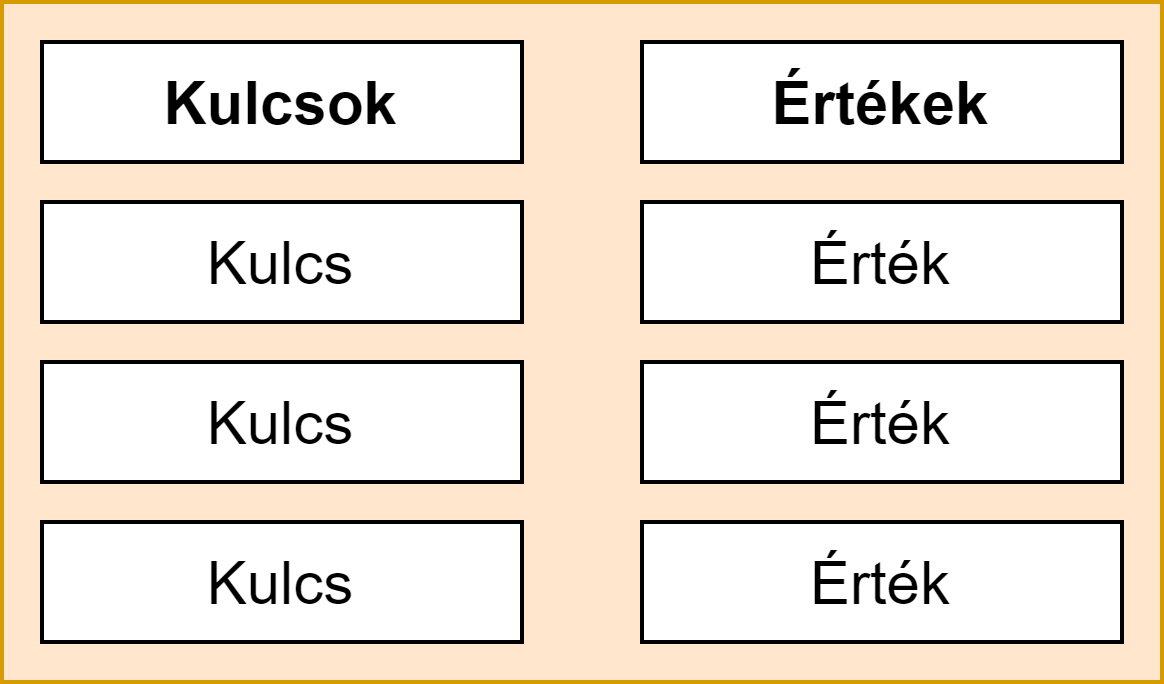
\includegraphics[scale=1]{images/paradigms/key-value.png}
    \caption{Kulcs-érték adatbázis}
    \label{fig:keyvalue}
\end{figure}

\subsection{Oszlopalapú adatbázis}

Az oszlopalapú adatbázis (vagy más néven oszlop- vagy oszlopcsalád adatbázis) hasonlít a kulcs-érték adatbázishoz, ugyanis itt is kulcs-érték páronként vannak tárolva az adatok, de az értékek oszlopokban kerülnek tárolásra. Egy oszlophoz jellemzően tartozik egy kulcs, egy érték, és opcionálisan egy időbélyeg. Nem tartozik hozzá séma, ezért csak szervezetlen (\textit{schema free}) adatok tárolására alkalmas. A CQL (\textit{Cassandra Query Language}) segítségével lehet lekérdezéseket írni, viszont nincsenek join műveletek. Ilyen adatbázisok például a Cassandra, az HBase és a BigTable. (\ref{fig:column}. ábra).

\begin{figure}[h]
    \centering
    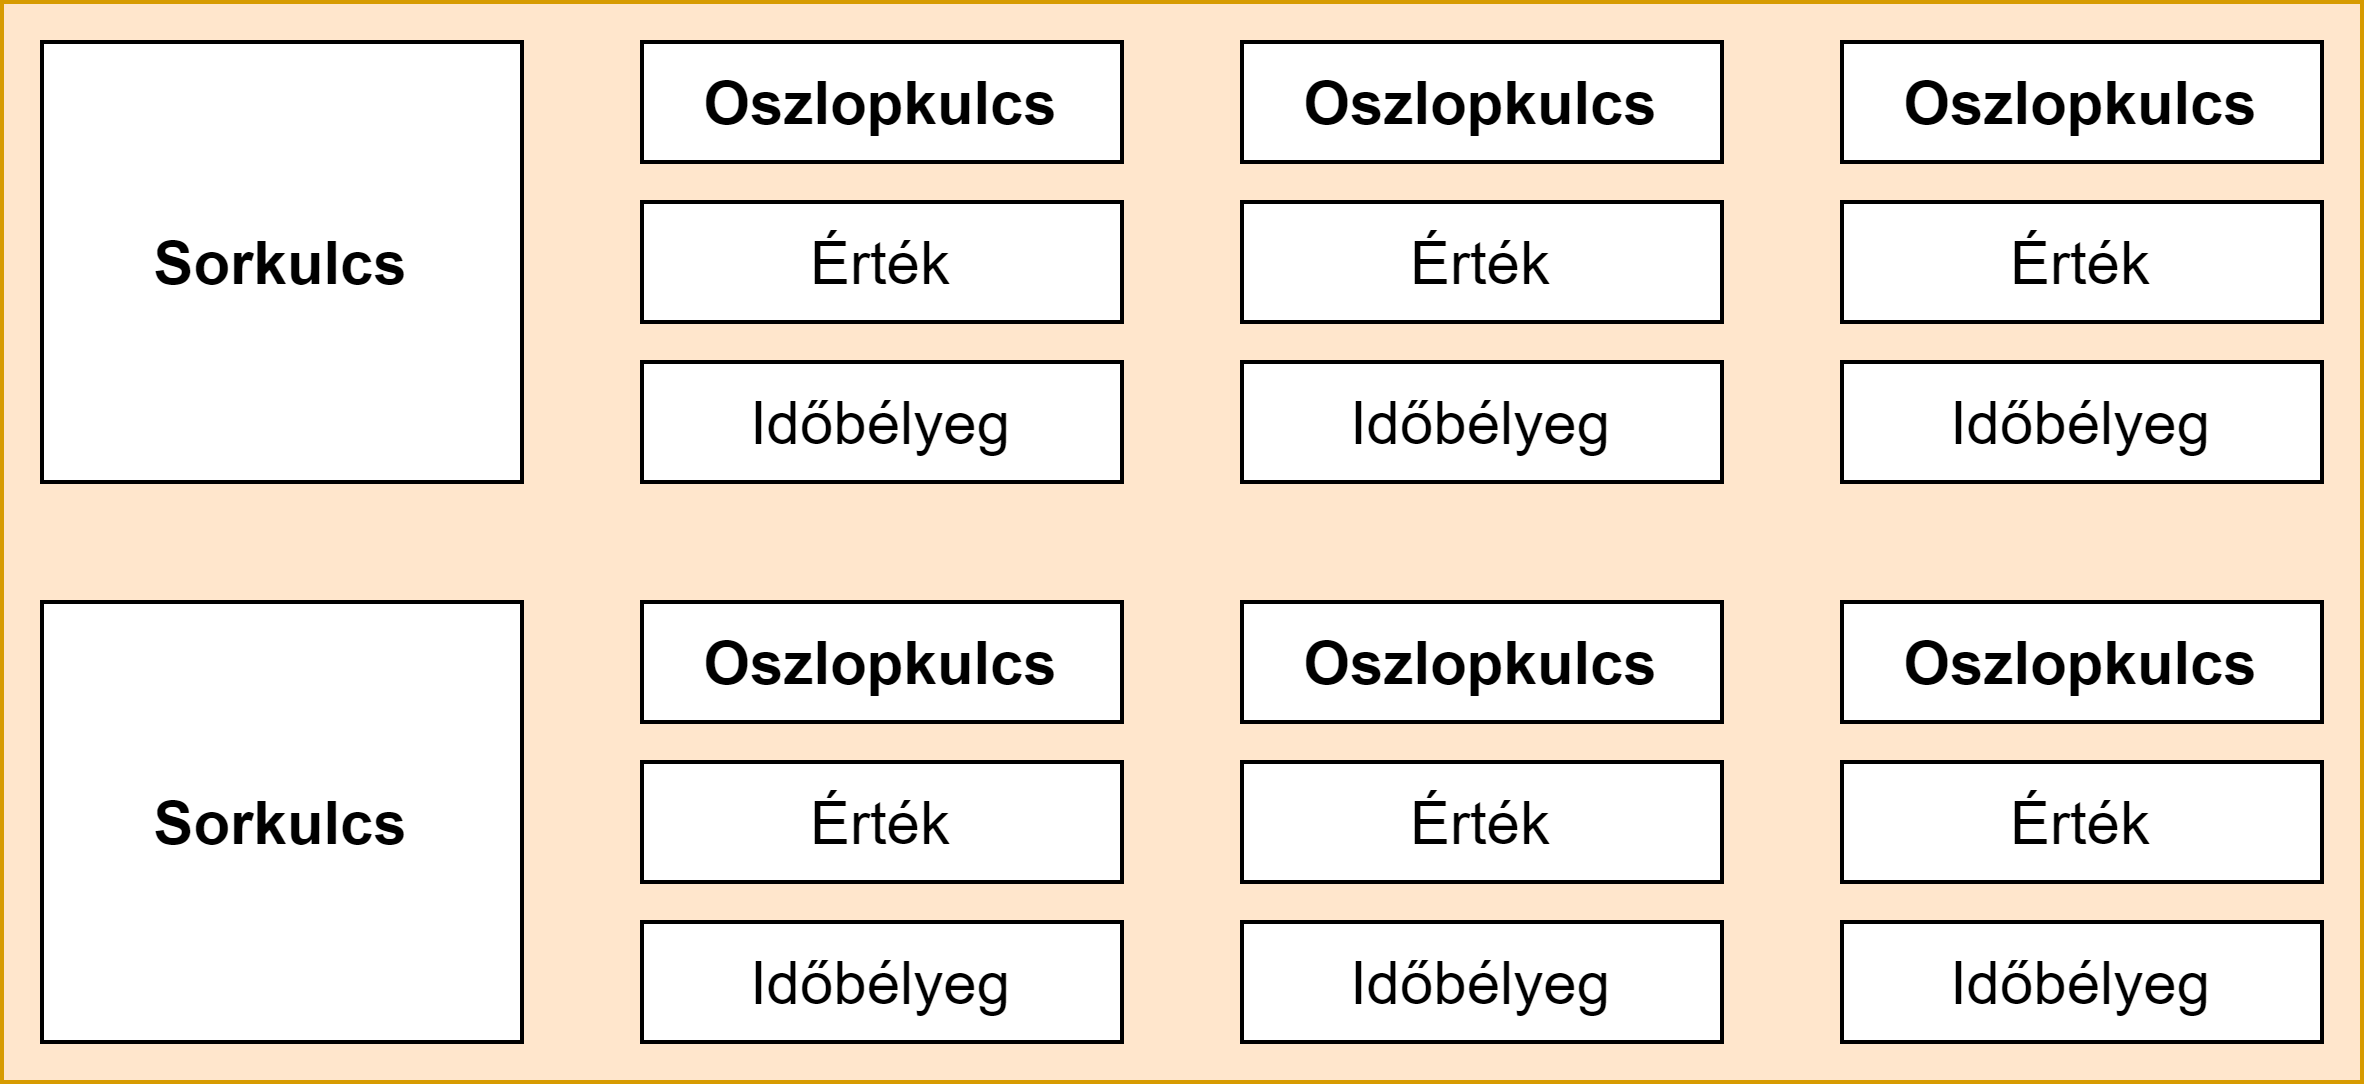
\includegraphics[scale=1]{images/paradigms/column.png}
    \caption{Oszlopalapú adatbázis}
    \label{fig:column}
\end{figure}

\subsection{Dokumentum adatbázis}

A dokumentum adatbázis dokumentumok tárolására és lekérdezésére szolgálnak. A dokumentumok önleíróak, hierarchikus szerkezetűek, kollekciókat és skalár értékeket tartalmazhatnak. A dokumentumok lehetnek például JSON, XML vagy YAML formátumokban. Ilyen adatbázisok például a MongoDB, a CouchDB és a Firestore.

\subsection{Relációs adatbázis}

A relációs adatbázis a relációs adatmodellen alapszik, amely az adatokat táblázatos elrendezésben kezeli. A rekordok ezen táblázatok sorai, a táblák sémája által definiált relációk elemei. Ilyen adatbázisok például az Oracle Database, a MySQL, MariaDB, PostgreSQL és a Microsoft SQL Server. (\ref{fig:relational}. ábra).

\begin{figure}[h]
    \centering
    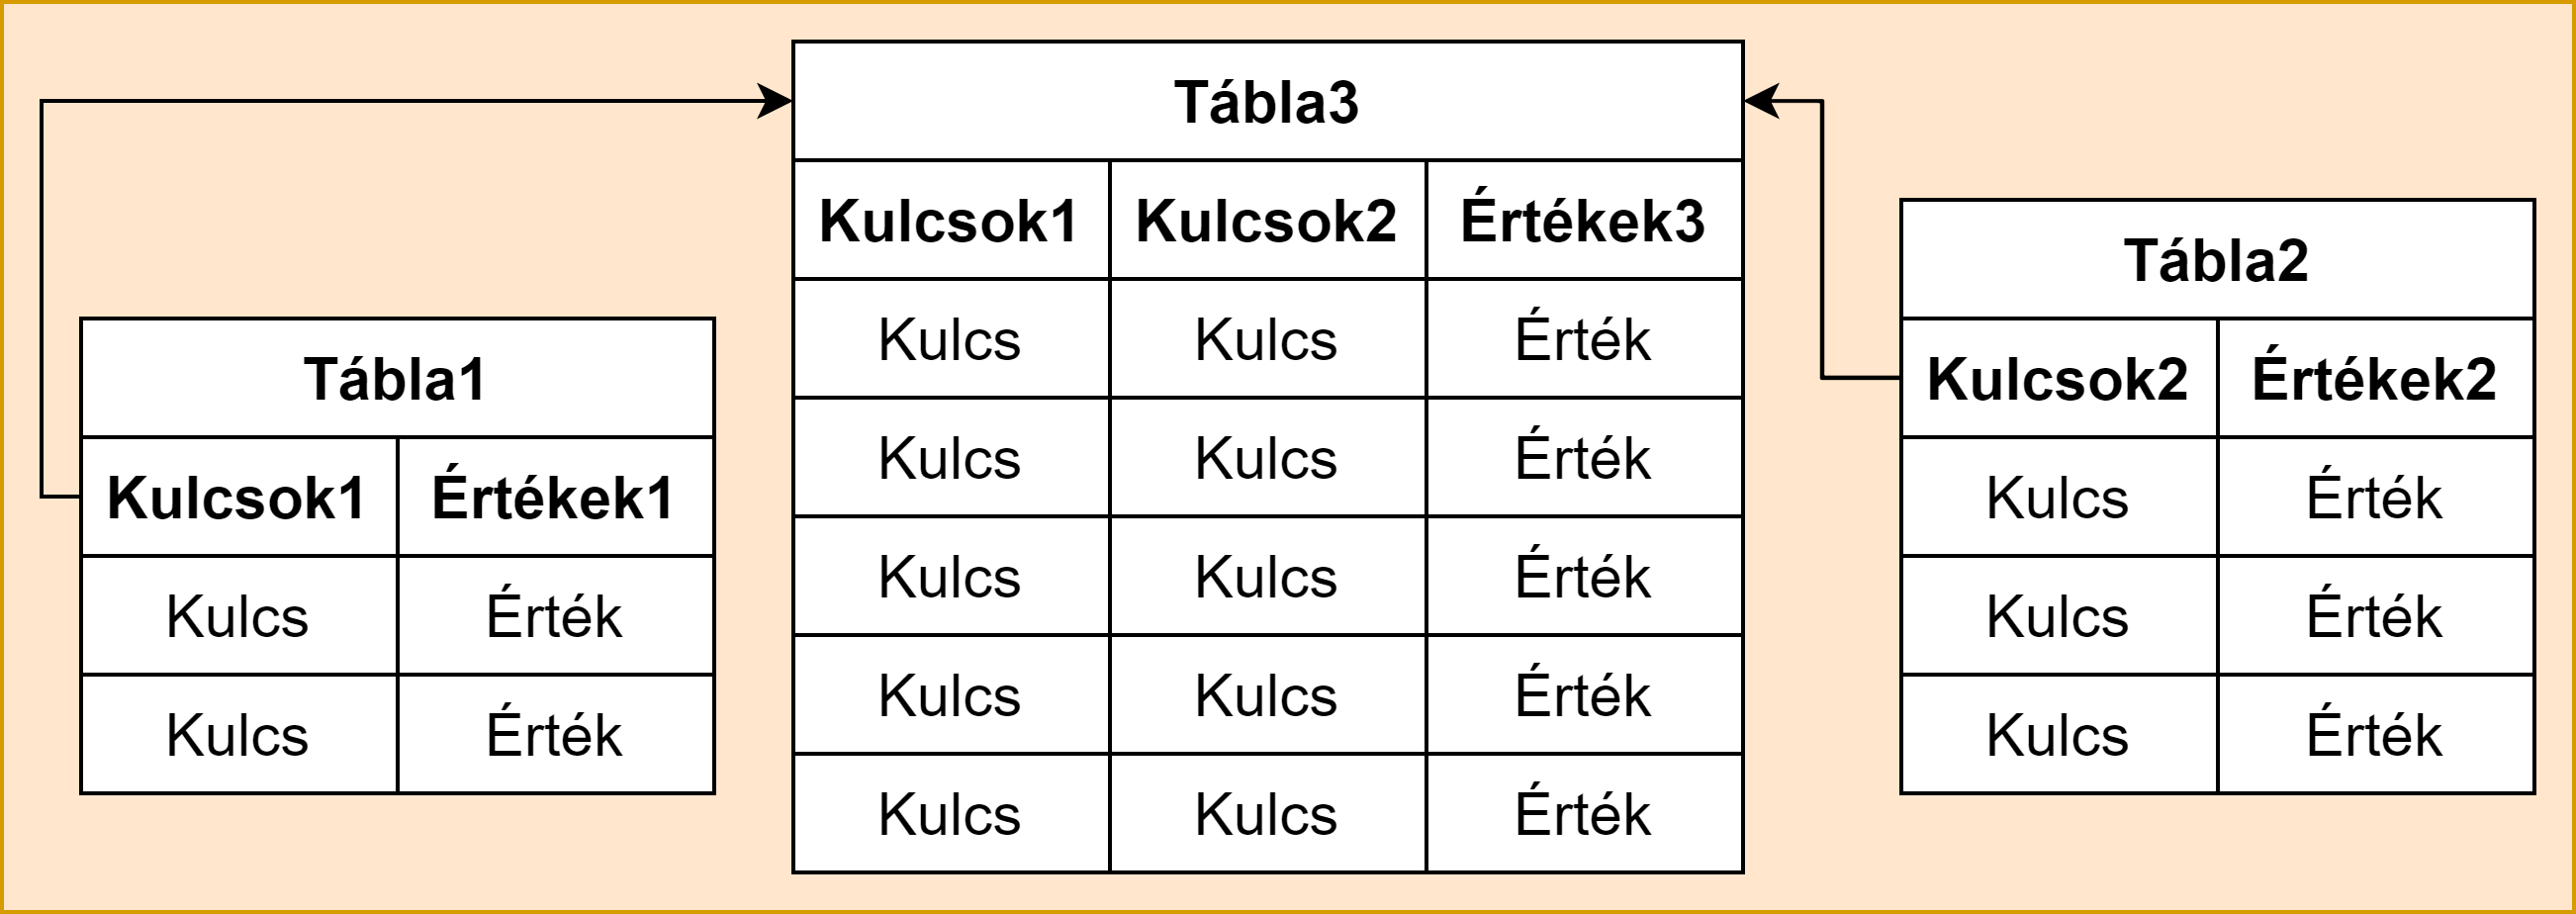
\includegraphics[scale=0.9]{images/paradigms/relational.png}
    \caption{Relációs adatbázis}
    \label{fig:relational}
\end{figure}

\subsection{Gráf adatbázis}

A gráf adatbázis gráfok hatékony tárolására és az azon végzett műveletek gyors végrehajtására ad lehetőséget. Az adatokat csomópontok és élek formájában tárolja. Jellemzően megvalósíthatóak benne komplex lekérdezések. Ilyen adatbázisok például a Neo4j, az Amazon Neptune és az Azure Cosmos DB. (\ref{fig:graph}. ábra).

\begin{figure}[h]
    \centering
    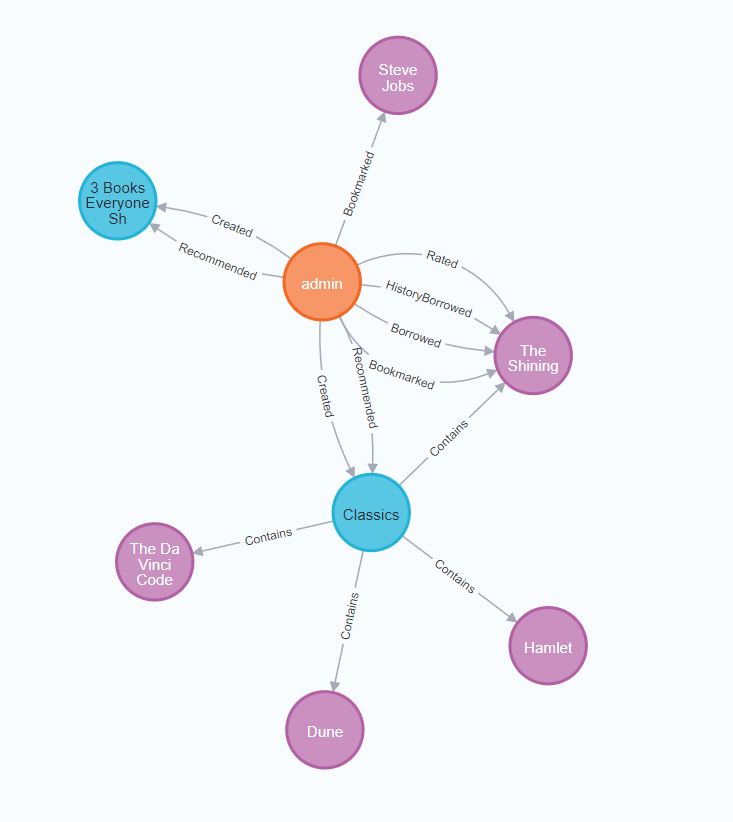
\includegraphics[scale=0.5]{images/paradigms/graph.png}
    \caption{Gráf adatbázis}
    \label{fig:graph}
\end{figure}


\subsection{Teljes szövegű kereső motor}

A teljes szövegű kereső motorra épülő adatbázisban a dokumentumok tartalmát indexelik. Az adatbázisban való kereséskor a keresés az indexen keresztül fog zajlani. Ilyen keresőmotorok például az Apache Lucene és az Elasticsearch.

\subsection{Több modelles adatbázis}

A több modelles adatbázis lehetőséget biztosít több fajta adatmodell együttes használatára. Ilyen adatbázisok például a Fauna és az ArangoDB.

\Section{Adatok leírása gráfokkal}

Gráfadatbázisok esetében az adatok csomópontok, és az azokat összekötő kapcsolatok formájában kerülnek tárolásra \cite{adatok-leirasa}. A csomópontokhoz és a kapcsolatokhoz tartozhatnak tulajdonságok is. Ezek kulcs-érték párok, amelyek az adott csomóponthoz vagy kapcsolathoz tartozó további információkat tárolják. A csomópontokat el lehet látni címkékkel is, amelyek így csoportosítják a csomópontokat. Általában a csomópont egy főnév, a kapcsolat egy ige.

\bigskip

Egy csomópont tulajdonságát bizonyos esetekben célszerű lehet külön csomópontként reprezentálni. Például egy gépjárműveket tartalmazó adatbázisban a gépjárművek márkáját lehetne tárolni tulajdonságként a gépjármű csomópontban, de célszerű lehet egy külön csomópontot létrehozni a márkának, köztük egy kapcsolattal.

\Section{Elterjedt gráfadatbázisok}

Számos elérhető gráfadatbázis szolgáltatás létezik. Ebben az alfejezetben röviden bemutatásra kerül közülük néhány.

\subsection{Neo4j}

A Neo4j a Neo4j, Inc. által fejlesztett gráfadatbázis \cite{neo4j}. Az architektúrát úgy tervezték, hogy az optimális legyen a csomópontok és a kapcsolatok kezelésére, tárolására és bejárására. Tulajdonsággráf (\textit{Property Graph}) megközelítést alkalmaz, amely előnyös amely előnyös a gráf bejárásának és a további műveletek elvégzésének futási ideje szempontjából. A Cypher lekérdező nyelvet használja, ami SQL jellegű.

\subsection{Amazon Neptune}

Az Amazon Neptune az Amazon.com, Inc. által fejlesztett gráfadatbázis \cite{neptune}. A Neptune egy gyors, megbízható és teljeskörű gráfadatbázis, amely megkönnyíti a szorosan összekapcsolt adatkészletekkel működő alkalmazások létrehozását és futtatását. A Neptune magja egy erre a célra épített, nagy teljesítményű gráf adatbázis motor. A motort több milliárd kapcsolat tárolására és az azok megjelenítéshez szükséges adatok ezredmásodperces késleltetéssel történő lekérdezésére optimalizálták. A Neptune támogatja az Apache TinkerPop Gremlin és a W3C SPARQL gráflekérdező nyelveit.

\subsection{Azure Cosmos DB}

Az Azure Cosmos DB a Microsoft Corporation által fejlesztett gráfadatbázis kezelő rendszer \cite{azure}. A kiadott lekérdezések jellemzően nagyon rövid válaszidővel adnak eredményt. A motor jó skálázhatóságot biztosít. 99,99\%-os SLA-t (\textit{Service-Level Agreement}/\textit{Szolgáltatási Szint Megállapodás}) kínál. Használható hozzá az Apache TinkerPop Gremlin lekérdező nyelv.

\subsection{Tigergraph}

A TigerGraph a TigerGraph által fejlesztett gráfadatbázis \cite{tigergraph}. A TigerGraph gyors adatbetöltési sebességet biztosít grafikonok készítéséhez. Lehetővé teszi a párhuzamos gráf-algoritmusok gyors végrehajtását, valós idejű frissítéseket és beillesztéseket REST API-n keresztül, valamint képes a valós idejű elemzések egyesítésére nagyszabású offline adatfeldolgozással. A GSQL szoftvert használja az adatbázis menedzselésére.

\subsection{AnzoGraph DB}

Az AnzoGraph DB a Cambridge Semantics által fejlesztett gráfadatbázis. Az AnzoGraph egy natív, masszívan párhuzamos feldolgozású gráf OLAP (\textit{Online Analytics Processing}) adatbázis \cite{anzograph1}, \cite{anzograph2}. Az adatok natív gráf formátumban kerülnek tárolásra a lemezen vagy a memóriában. A gráf OLAP technológia lehetővé teszi a felhasználók számára a grafikonok adatainak interaktív megtekintését, elemzését és frissítését. Használhatóak hozzá a SPARQL és a Cypher lekérdező nyelvek.

\subsection{Dgraph}

A Dgraph a Dgraph Labs által fejlesztett gráfadatbázis \cite{dgraph}. A Dgraph egy horizontálisan skálázható. A Dgraph a modern alkalmazások és webhelyek működéséhez szükséges nagy tranzakciós terhelésre készült. A GraphQL lekérdező nyelvre épülő DQL-t (\textit{Dgraph Query Language}) használja.
